\documentclass[border=3mm]{standalone}
\usepackage{tikz}
\begin{document}
	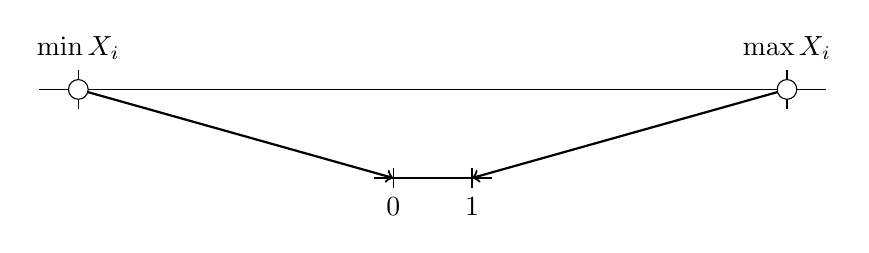
\begin{tikzpicture}[scale=0.5]
		\draw (-10,0)-- (10,0); %Axis
		\draw (-9,-0.5)--(-9,0.5) node[above] {$\min{X_i}$};
		\draw (9,-0.5)--(9,0.5) node[above] {$\max{X_i}$};
		\draw (-1,-2.)--(-1,-2.5)  node[below]{0};
		\draw (1, -2)--(1,-2.5) node[below]{1};
		\draw[->,thick] (-9,0) --(-1,-2.25) {};
		\draw[->,thick] (9,0)--(1,-2.25){};
		\draw(-1.5,-2.25)--(1.5,-2.25);
		\draw[fill=white] (-9,0) circle (0.25);
		\draw[fill=white] (9,0) circle (0.25);
	\end{tikzpicture}
\end{document}